%%%%%%%%%%%%%%%%%%%%%%%%%%%%%%%%%%%%%%%%%%%%%%%%%%%%%%%%%%%%%%%%%%%%%%%%%%%%%%%
%\documentclass[12pt]{article}
%\documentclass[12pt]{scrartcl}
\documentclass{hitec} % contained in texlive-latex-extra
\settextfraction{0.9} % indent text
\usepackage{csquotes}
\usepackage[hidelinks]{hyperref} % doi links are short and usefull?
\hypersetup{%
    colorlinks=true,
    linkcolor=blue,
    urlcolor=magenta
}
\urlstyle{rm}
\usepackage[english]{babel}
\usepackage{mathtools} % loads and extends amsmath
\usepackage{amssymb}
% packages not used
%\usepackage{graphicx}
%\usepackage{amsthm}
%\usepackage{subfig}
\usepackage{bm}
\usepackage{longtable}
\usepackage{booktabs}
\usepackage{ragged2e} % maybe use \RaggedRight for tables and literature?
\usepackage[table]{xcolor} % for alternating colors
%\rowcolors{2}{gray!25}{white} %%% Use this line in front of longtable
\renewcommand\arraystretch{1.3}
\usepackage[most]{tcolorbox}
\usepackage{doi}
\usepackage[sort,square,numbers]{natbib}
\bibliographystyle{abbrvnat}
%%% reset bibliography distances %%%
\let\oldthebibliography\thebibliography
\let\endoldthebibliography\endthebibliography
\renewenvironment{thebibliography}[1]{
  \begin{oldthebibliography}{#1}
    \RaggedRight % remove if justification is desired
    \setlength{\itemsep}{0em}
    \setlength{\parskip}{0em}
}
{
  \end{oldthebibliography}
}
%%% --- %%%

\definecolor{light-gray}{gray}{0.95}
\newcommand{\code}[1]{\colorbox{light-gray}{\texttt{#1}}}
\newcommand{\eps}{\varepsilon}
\renewcommand{\d}{\mathrm{d}}
\renewcommand{\vec}[1]{{\boldsymbol{#1}}}
\newcommand{\dx}{\,\mathrm{d}x}
%\newcommand{\dA}{\,\mathrm{d}(x,y)}
%\newcommand{\dV}{\mathrm{d}^3{x}\,}
\newcommand{\dA}{\,\mathrm{dA}}
\newcommand{\dV}{\mathrm{dV}\,}

\newcommand{\Eins}{\mathbf{1}}

\newcommand{\ExB}{$\bm{E}\times\bm{B} \,$}
\newcommand{\GKI}{\int d^6 \bm{Z} \BSP}
\newcommand{\GKIV}{\int dv_{\|} d \mu d \theta \BSP}
\newcommand{\BSP}{B_{\|}^*}
\newcommand{\Abar}{\langle A_\parallel \rangle}
%Averages
\newcommand{\RA}[1]{\left \langle #1 \right \rangle} %Reynolds (flux-surface) average
\newcommand{\RF}[1]{\widetilde{#1}} %Reynolds fluctuation
\newcommand{\FA}[1]{\left[\left[ #1 \right]\right]} %Favre average
\newcommand{\FF}[1]{\widehat{#1}} %Favre fluctuation
\newcommand{\PA}[1]{\left \langle #1 \right\rangle_\varphi} %Phi average

%Vectors
\newcommand{\ahat}{\bm{\hat{a}}}
\newcommand{\bhat}{\bm{\hat{b}}}
\newcommand{\chat}{\bm{\hat{c}}}
\newcommand{\ehat}{\bm{\hat{e}}}
\newcommand{\bbar}{\overline{\bm{b}}}
\newcommand{\xhat}{\bm{\hat{x}}}
\newcommand{\yhat}{\bm{\hat{y}}}
\newcommand{\zhat}{\bm{\hat{z}}}

\newcommand{\Xbar}{\bar{\vec{X}}}
\newcommand{\phat}{\bm{\hat{\perp}}}
\newcommand{\that}{\bm{\hat{\theta}}}

\newcommand{\eI}{\bm{\hat{e}}_1}
\newcommand{\eII}{\bm{\hat{e}}_2}
\newcommand{\ud}{\mathrm{d}}

%Derivatives etc.
\newcommand{\pfrac}[2]{\frac{\partial#1}{\partial#2}}
\newcommand{\ffrac}[2]{\frac{\delta#1}{\delta#2}}
\newcommand{\fixd}[1]{\Big{\arrowvert}_{#1}}
\newcommand{\curl}[1]{\nabla \times #1}

\newcommand{\np}{\vec{\nabla}_{\perp}}
\newcommand{\npc}{\nabla_{\perp} \cdot }
\newcommand{\nc}{\vec\nabla\cdot}
\newcommand{\cn}{\cdot\vec\nabla}
\newcommand{\vn}{\vec{\nabla}}
\newcommand{\npar}{\nabla_\parallel}

\newcommand{\GAI}{\Gamma_{1}^{\dagger}}
\newcommand{\GAII}{\Gamma_{1}^{\dagger -1}}
\newcommand{\T}{\mathrm{T}}
\newcommand{\Tp}{\mathcal T^+_{\Delta\varphi}}
\newcommand{\Tm}{\mathcal T^-_{\Delta\varphi}}
\newcommand{\Tpm}{\mathcal T^\pm_{\Delta\varphi}}
%%%%%%%%Some useful abbreviations %%%%%%%%%%%%%%%%
\def\feltor{{\textsc{Feltor }}}

\def\fixme#1{\typeout{FIXME in page \thepage :{#1}}%
 \textsc{\color{red}[{#1}]}}


%%%%%%%%%%%%%%%%%%%%%%%%%%%%%%%%%%%%%%%%%%%%%%%%%%%%%%%%%%%%%%%%%%%%%%%%%%%%%%%
\begin{document}
%\preprint{}

\title{Streamline integration as a method for two-dimensional elliptic grid generation}
\author{M.~Wiesenberger, M.~Held, and L.~Einkemmer}
%\email{Matthias.Wiesenberger@uibk.ac.at}
%\affiliation{Institute for Ion Physics and Applied Physics, Association EURATOM-\"OAW,  University of
%   Innsbruck, A-6020 Innsbruck, Austria}
%\affiliation{Institute for Ion Physics and Applied Physics, Association EURATOM-\"OAW,  University of
   %Innsbruck, A-6020 Innsbruck, Austria}
%\address{Institute for Ion Physics and Applied Physics,  Universit\"at 
   %Innsbruck,  A-6020 Innsbruck, Austria}
%\address{Numerical Analysis group,  Universit\"at Innsbruck, A-6020 Innsbruck, Austria}
 
\maketitle
\begin{abstract}
  [This writeup is based/copied on the recent article \cite{Wiesenberger2017}] \\
We propose a new numerical algorithm to construct a structured
numerical elliptic grid of a doubly connected domain. Our method is 
applicable to domains with boundaries defined by two contour lines of a two-dimensional function. 
Furthermore, we can adapt any analytically given boundary
aligned structured
grid, which specifically includes polar and Cartesian grids.
The resulting coordinate lines are orthogonal to the boundary. 
Grid points as well as
the elements of the Jacobian matrix can be computed efficiently and up to machine precision. 
In the simplest case we construct conformal grids, yet with the help of weight functions and monitor metrics we can control the
distribution of cells across the domain. 
Our algorithm is parallelizable and easy to implement with
elementary numerical methods. 
We assess the quality of grids by considering both the distribution of cell sizes and the accuracy of the solution to 
elliptic problems. 
Among the tested grids these key properties are best fulfilled by the grid constructed with the monitor metric approach.
%All in all, the grid constructed with a monitor metric
%yields the best accuracy and cell sizes compared

%Simple flux aligned orthogonal grids are suitable for the solution
%of flux aligned problems, but they exhibit 
%very large ratios of maximal to minimal cell size. 
%If we construct a conformal grid, the aspect ratio of the cells is constant by construction. However, the variation in cell size is large 
%and the errors of the elliptic equation are high. 
%The adapted grid and the grid with monitor metric yield smaller variation in size and smaller errors, where
%the monitor grid overall has the smallest ratios of maximal to minimal cell size.
%The errors and cell sizes are competitive with a previously suggested near conformal grid.
%
%It is based on the integration of the streamlines of the two vector fields that
%form the basis of the coordinate system. 
%These vector fields are either built directly from the given function or from the solution of a suitably chosen elliptic equation (which 
%can be solved once an initial grid has been constructed). 
%We are able to construct conformal, orthogonal and curvilinear coordinates.
%The method is parallelizable and the metric elements can be computed with high accuracy. 
%Furthermore, it is easy to implement as only the integration 
%of well-behaved ordinary differential equations and the inversion
%of a linear elliptic equation are required.
%All our grids are orthogonal to the boundary of the domain, which is the major
%advantage over previously suggested grids. 
\end{abstract}

\section{High precision elliptic grid generation} \label{sec:geometry}

Given is a function $\psi(x,y)$ in Cartesian coordinates. 
We want to construct a grid on the region 
bounded by the two lines
$\psi(x,y) = \psi_0$ and $\psi(x,y)=\psi_1$ with $\psi_0\neq\psi_1$.
The derivative of the function $\psi$ may not vanish within this region and on the boundary and 
we further assume that the region is topologically a ring. 
Note here that this excludes the description of domains with an X-point (saddle point) or O-point (local extremum). 
The numerical grid is described by a mapping of the discretization of the rectangular
computational domain $(u,v) \in [0,u_1]\times[0,2\pi]$ to the physical domain $(x,y)$. $u_1$ is an unknown, which the grid generation process has to provide. 

%Together with 
%this mapping described by $x_i = x(u_i, v_i),\ y_i = y(u_i, v_i)$ we construct the derivatives
%$u_x(u_i,v_i),\ v_x(u_i, v_i),\ u_y(u_i, v_i),\ v_y(u_i,v_i)$ in order to 
%transform tensors to the curvilinear coordinate system. 
%Here and in the following we use the notation $u_x\equiv \frac{\partial u}{\partial x}$.
%The index $i$ is given by $i=0,1,\dots N_uN_v$, where $N_u$ and $N_v$ are the number of points
%in $u$ and $v$ respectively. The discretization of the computational domain need 
%not be equidistant. We will for example use the Gauss-Legendre nodes 
%needed for a discontinuous Galerkin discretization. 
%%%%%%%%%%%%%%%%%%%%%%%%%%%%%%%%%%%%%%%%%%%%%%%%%%%%%%%%%%%%%%%%%
\begin{figure}[htbp]
\centering
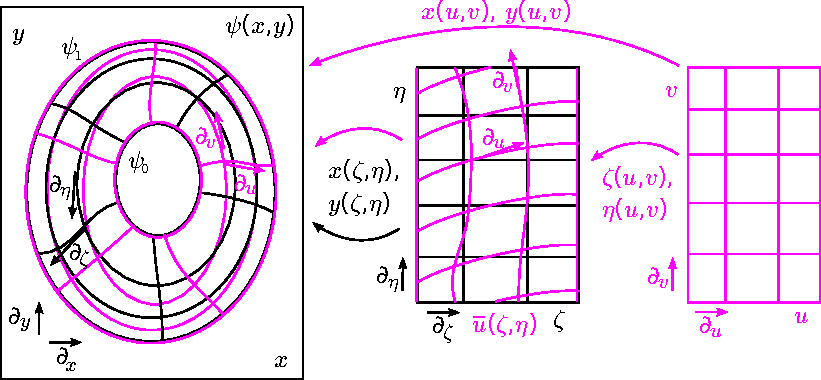
\includegraphics[trim = 0px 0px 0px 0px, clip, scale=1.0]{./drawing_magenta}
\caption{
  Sketch of the coordinate systems, coordinate lines and basis vector fields 
  involved in our method.
}
\label{fig:sketch}
\end{figure}
%%%%%%%%%%%%%%%%%%%%%%%%%%%%%%%%%%%%%%%%%%%%%%%%%%%%%%%%%%%%%%%%%
As mentioned in the introduction and illustrated in Fig.~\ref{fig:sketch} the idea of our algorithm are two consecutive coordinate transformations constructed by streamline integration. 
We denote the first transformation with $x(\zeta, \eta)$, $y(\zeta, \eta)$, where
the $\zeta$ coordinate is aligned with $\psi$ and $\eta$ is an angle-like coordinate. The solution of the 
elliptic equation on this flux-aligned coordinate system is denoted with $\bar u(\zeta, \eta)$. 
The second coordinate transformation is then denoted $\zeta(u,v)$, $\eta(u,v)$ with $u$ aligned to $\bar u$.

When deriving the algorithm we use basic methods and notational 
conventions of differential geometry.  
Here, we recommend the excellent Reference~\cite{Frankel} as an introduction to the topic.  
We do so since in this approach the separate roles of the metric tensor, 
the coordinate system and its base vector fields are very clear. This is 
paramount for a concise description of our method. 


In this Section we first show how the
basis vector fields can be integrated to construct coordinate lines
 with the example of orthogonal coordinates in Section~\ref{sec:orthogonal}. This follows
an introduction of some helpful quantities, our notation and streamlines
in Section~\ref{sec:preliminaries}. 
%In Section~\ref{sec:orthogonal} we review the
%construction of orthogonal coordinates via the integration of 
%streamlines, that is ordinary differential 
%equations. 
In the next step we transform, discretize and solve an elliptic equation on the flux aligned
coordinate system.
The solution $\bar u(\zeta, \eta)$ then takes the role of a new flux function in the flux aligned coordinates. 
We can therefore repeat the streamline integration method in the flux aligned
coordinate system in order to construct coordinate lines of the final $u,v$ coordinates.
We discuss three examples of this method.
%In Section~\ref{sec:laplace} we discretize and 
%solve the Laplace equation.
%with local discontinuous Galerkin (dG) methods. 
In 
Section~\ref{sec:conformal} we consider the simple Laplace and the Cauchy-Riemann equations~\eqref{eq:CR}
in order to construct conformal coordinates.
In Section~\ref{sec:adaption} we modify the elliptic equation to allow grid adaption, before
we introduce the monitor metric in Section~\ref{sec:metric}. 
Finally, we present our algorithm in Section~\ref{sec:elliptic}. 

\subsection{Preliminaries} \label{sec:preliminaries}
In a curvilinear
coordinate system $(\zeta,\eta)$ the components of the metric tensor and its inverse
take the form 
\begin{align}
  \vec g(\zeta,\eta) = \begin{pmatrix}
    g_{\zeta\zeta} & g_{\zeta\eta}  \\
    g_{\zeta\eta} & g_{\eta\eta}  
  \end{pmatrix}
  \quad
  \vec g^{-1}(\zeta,\eta) = \begin{pmatrix}
    g^{\zeta\zeta} & g^{\zeta\eta}  \\
    g^{\zeta\eta} & g^{\eta\eta}  
  \end{pmatrix}
  \label{}
\end{align}
We denote $g = \det{\vec g} = g_{\zeta\zeta}g_{\eta\eta}-g_{\zeta\eta}^2$.
For Cartesian coordinates $(x,y)$ the elements of the inverse metric tensor are 
transformed by
\begin{subequations}
\begin{align}
  g^{\zeta\zeta} &=  \zeta_x^2+\zeta_y^2\\
  g^{\zeta\eta} &=  \zeta_x \eta_x+\zeta_y \eta_y\\
  g^{\eta\eta} &=  \eta_x^2+\eta_y^2
  \label{}
\end{align}
\end{subequations}
since $g^{xx}=g^{yy}=1$ and $g^{xy}=0$. 
Given $\zeta(x,y)$, $\eta(x,y)$ and its inverse $x(\zeta,\eta)$, $y(\zeta,\eta)$ recall that their Jacobian matrices are related by
\begin{align}
  \begin{pmatrix}
    x_\zeta & x_\eta \\
    y_\zeta & y_\eta
  \end{pmatrix} \bigg\rvert_{\zeta(x,y),\eta(x,y)}
  =
  \frac{1}{\zeta_x\eta_y - \zeta_y\eta_x }\begin{pmatrix}
    \eta_y & -\zeta_y \\
    -\eta_x & \zeta_x
  \end{pmatrix}\bigg\rvert_{x,y} 
  \label{eq:inverse}
\end{align}
With the rules of tensor transformation it is easy to prove that the element of the volume form $\sqrt{g}$ is related to the Jacobian via
\begin{align}
  %\mathcal V^2:=\d x\wedge \d y = (x_uy_v - y_ux_v)\d u\wedge\d v = \frac{\d u\wedge\d v}{u_xv_y - u_yv_x} \equiv \sqrt{g} \d u\wedge \d v
%\iint \d V:= \iint \d x \d y = \iint (x_uy_v - y_ux_v)\d u\d v &=  \nonumber\\
%\iint\frac{\d u\d v}{u_xv_y - u_yv_x} &\equiv \iint \sqrt{g} \d u\d v
\sqrt{g} = (x_\zeta y_\eta-y_\zeta x_\eta) = (\eta_y\zeta_x -\eta_x\zeta_y)^{-1}
  \label{eq:vol}
\end{align}
The components of the gradient operator and the divergence in an arbitrary coordinate
system read
\begin{subequations}
\begin{align}
  \left( \nabla f \right)^i &= g^{ij}\partial_j f \\
  \nabla \cdot \vec A &= \frac{1}{\sqrt g}\partial_i \left( \sqrt{g} A^i  \right),
\end{align}
  \label{eq:arbitrary}
\end{subequations}
where we sum over repeated indices $i,j\in\{\zeta,\eta\}$ and define $\partial_\zeta \equiv \partial/\partial \zeta$, $\partial_\eta \equiv \partial/\partial \eta$.
%Note that 
%\begin{align}
%  \d x = x_R \d R + x_Z \d Z\\
%  \d y = y_R \d R + y_Z \d Z
%  \label{}
%\end{align}
%and
%\begin{align}
%  \partial_x = R_x \partial_R + Z_x \partial_Z\\
%  \partial_y = R_y \partial_R + Z_y \partial_Z
%  \label{}
%\end{align}
%Figuratively $\d x$ and $\d y$ are the one-forms that form the lines of constant $x$ and $y$, while the coordinate lines are given by the streamlines of $\partial_x$ and $\partial_y$.
%Recall that the coordinate line $x$ is implicitly defined by the points with $y=const$ and vice versa\cite{Frankel}. 
% Through the inverse derivatives
%Eq.~\eqref{eq:inverse} $\partial_y$ is related with $\d x$ and $\partial_x$ is 
%related with $\d y$. 
%
%The contravariant vectors $\nabla x$ and $\nabla y$ are the vectors that are everywhere perpendicular to $\d x$ and $\d y$. 
%$\nabla x$ and $\nabla y$ are in general not parallel to $\partial_x$ and $\partial_y$, yet\footnote{ Some textbooks use the notation $e_x = \partial_x$ and $e^x=\nabla x$}
%\begin{align}
% \partial_y \cdot \nabla y = \partial_x \cdot \nabla x = 1\\
% \partial_x \cdot \nabla y = \partial_y \cdot \nabla x =0
%  \label{}
%\end{align}
%Now note that in order to reconstruct $R(x,y)$, $Z(x,y)$ we have to integrate the 
%coordinate lines i.e. $\partial_x$ and $\partial_y$.
Finally, we introduce the 
geometrical poloidal angle 
\begin{align}
  \theta (x,y) = \begin{cases}
    +\arccos\left( \frac{x-x_0}{\sqrt{(x-x_0)^2 + (y-y_0)^2}} \right) \text{ for } y\geq y_0 \\
    -\arccos\left( \frac{x-x_0}{\sqrt{(x-x_0)^2 + (y-y_0)^2}} \right) \text{ for } y< y_0 
  \end{cases}
  \label{eq:deftheta}
\end{align}
such that the differential 1-form
\begin{align}
  \d \theta = 
    -\frac{y-y_0}{(x-x_0)^2+(y-y_0)^2} \d x
    +\frac{x-x_0}{(x-x_0)^2+(y-y_0)^2} \d y,
  \label{eq:theta}
\end{align}
where $(x_0,y_0)$ is any point inside the region bounded by $\psi_0$.

Streamline integration is the central part of our algorithm. Recall that
given a vector field $v(x,y)=v^x(x,y)\partial_x + v^y(x,y)\partial_y$ its streamlines are given by the equation
\begin{subequations}
\begin{align}
  \frac{\d x}{\d t } = v^x(x,y)|_{x(t), y(t)} \\
  \frac{\d y}{\d t } = v^y(x,y)|_{x(t), y(t)}
\end{align}
\label{eq:streamlines}
\end{subequations}
where $t$ is a parameter. Recall here that in differential geometry 
the directional derivatives $\partial_x$ and
$\partial_y$ are the base vector fields of the coordinate system\footnote{ 
  Some textbooks (e.g.~\cite{haeseleer}) introduce the notation $\vec e_i := \partial \vec x /\partial x^i$ 
  and $\vec e^i := \nabla x^i$. 
  While this formulation is suitable in many situations we refrain from 
  using it since it mixes the metric into the basis vectors through the use of 
  the gradient (cf. Eq.~\eqref{eq:arbitrary}). 
  This is unpractical for our purposes.}.
Now recall that if we have a function $f(x,y)$ 
such that $f(x(t), y(t))$ is a one-to-one map from $t$ to $f$ we can re-parameterize
Eq.~\eqref{eq:streamlines} by
\begin{subequations}
\begin{align}
  \frac{\d x}{\d f } = \frac{\d x/\d t|_{t(f)}}{\d f/\d t|_{t(f)}} = 
  \frac{v^x(x,y) }{ (v^x\partial_xf + v^y\partial_yf)(x,y) }\bigg |_{x(f), y(f)}\\
  \frac{\d y}{\d f } = \frac{\d y/\d t|_{t(f)}}{\d f/\d t|_{t(f)}} = 
  \frac{v^y(x,y) }{ (v^x\partial_xf + v^y\partial_yf)(x,y) }\bigg |_{x(f), y(f)}
\end{align}
\label{eq:reparameter}
\end{subequations}
Furthermore, the derivative of any function $g(x,y)$ along the streamlines of $v$ 
parameterized by $f$ reads
\begin{align}
  \frac{\d g}{\d f }\bigg |_{x(f),y(f)} = 
  \frac{(v^x\partial_x g + v^y\partial_y g)(x,y) }{ (v^x\partial_xf + v^y\partial_yf)(x,y) }\bigg |_{x(f),y(f)}
  \label{}
\end{align}


Figuratively, in any coordinate system $(\zeta,\eta)$ the 1-forms $\d \zeta$ and $\d \eta$ (the contravariant basis) are visualized by the lines (surfaces in higher dimensions) 
of constant $\zeta$ and $\eta$. 
At the same time the streamlines of the vector fields $\partial_\zeta$ and $\partial_\eta$ (the covariant basis) 
give the coordinate lines of $\zeta$ and $\eta$ (cf. Fig.~\ref{fig:sketch}). 
For example, if we hold $\eta$ constant and vary $\zeta$, we go along a streamline of 
$\partial_\zeta$. This implies that in two dimensions $\d \eta$ and $\partial_\zeta$ 
trace the same line. The vector fields $\nabla \zeta$ and $\nabla \eta$ are associated to 
$\d \zeta$ and $\d \eta$ through the metric tensor by Eq.~\eqref{eq:arbitrary} and are the vector fields that
are everywhere perpendicular to the lines of constant $\zeta$ and $\eta$, respectively. 
It is important to realize that in general curvilinear coordinates the vector
fields $\nabla \zeta$ and $\nabla \eta$ point in 
different directions than $\partial_\zeta$ and $\partial_\eta$.
The central point in our algorithm is the realization that once we can 
express $\partial_\zeta$ and $\partial_\eta$ in terms of $\partial_x$ and 
$\partial_y$ we can immediately construct the coordinate transformation 
by integrating 
streamlines of $\partial_\zeta$ and $\partial_\eta$ using Eq.~\eqref{eq:streamlines}. This 
holds true even if $(x,y)$ were curvilinear coordinates. The components of the 
one-forms $\d \zeta$ and $\d\eta$ in terms of $\d x$ and $\d y$ form 
the elements of the Jacobian matrix of the transformation. These 
are also necessary in order to transform any tensor (including the metric) 
from the old to the new coordinate system. 


\subsection{Orthogonal coordinates} \label{sec:orthogonal}
In general, orthogonal coordinates $\zeta, \eta$ with $\zeta$ aligned to $\psi$ are described by
\begin{subequations}
\begin{align}
  \d \zeta & = \zeta_x\d x +\zeta_y\d y =  f(\psi)(\psi_x \d x + \psi_y \d y) \\
  \d \eta  & = \eta_x \d x + \eta_y \d y = h(x,y) ( -\psi_y \d x + \psi_x \d y)
\end{align}
  \label{eq:orthogonal}
\end{subequations}
With Eq.~\eqref{eq:orthogonal} we have $g^{\zeta\eta} = \zeta_x\eta_x + \zeta_y\eta_y = 0$,
$g^{\zeta\zeta} = (\nabla\psi)^2 f^2$, $g^{\eta\eta} = (\nabla\psi)^2h^2$ and $\sqrt{g}^{\,-1} = (\nabla\psi)^2 h f$. 
From Eq.~\eqref{eq:inverse} we directly see that the basis vector fields are
\begin{subequations}
\begin{align}
  \partial_\zeta&= x_\zeta\partial_x + y_\zeta\partial_y = \frac{1}{(\nabla\psi)^2f} (\psi_x \partial_x + \psi_y\partial_y) \\
  \partial_\eta &=  x_\eta\partial_x + y_\eta\partial_y =  \frac{1}{(\nabla\psi)^2h} (-\psi_y \partial_x + \psi_x\partial_y) 
\label{eq:orthogonal_linesb}
\end{align}
\label{eq:orthogonal_lines}
\end{subequations}
i.e. $\partial_\zeta$ points into the direction of the gradient of $\psi$ and $\partial_\eta$ into the direction of constant $\psi=\text{const}$ surfaces.
Now, the coordinate system is defined up to the functions $f(\psi)$ and $h(x,y)$.
Note that $f$ must be a function of $\psi$ only since the restriction $\d(\d \zeta)=0$ must hold.
Furthermore, $f(\psi) = \d\zeta/ \d\psi \neq 0 $ is in principle an arbitrary function, yet we choose $f(\psi) = f_0 = \text{const}$.
With this choice we directly get
\begin{align}
  \zeta(x,y) = f_0(\psi(x,y)-\psi_0)
  \label{eq:zeta}
\end{align}
Note that $\zeta_0=0$ and $\zeta_1=f_0(\psi_1-\psi_0)$.
The up to now undefined function $h(x,y)$ is not arbitrary since $\d(\d \eta) = 0$ must hold. This is the requirement that $\d \eta$ must be
a closed form in order for the potential $\eta$ to exist. 
We can express this as
\begin{align}
  (\psi_x\partial_x + \psi_y\partial_y) h = f(\nabla\psi)^2 \partial_\zeta h= -h\Delta \psi 
  \label{eq:hequation}
\end{align}
where $\Delta \psi = \psi_{xx} + \psi_{yy}$ is the two-dimensional Laplacian.
Let us remark here that Eq.~\eqref{eq:hequation} can be written as $\nabla\cdot\left( h\nabla\psi \right)=0$, which makes the orthogonal grid an elliptic grid
with adaption function $h$ as becomes evident later. 
In order to integrate this equation we need an initial condition for $h$. 
We choose to first discretize the line given by $\psi(x,y) = \psi_0$. 

As already mentioned $\partial_\eta$ is the vector field the streamlines of which give the 
coordinate lines for $\eta$. We choose $h(x,y) = \text{const}$ on $\psi_0$. To this end
we parameterize the coordinate line by $\theta$ (cf. Eq.~\eqref{eq:reparameter})
\begin{subequations}
\begin{align}
  \left . \frac{\d x}{\d \theta}\right|_{\zeta=0}=\frac{x_\eta}{\theta_\eta} = \frac{-\psi_y}{\psi_x\theta_y - \psi_y \theta_x}\\
  \left . \frac{\d y}{\d \theta}\right|_{\zeta=0}=\frac{y_\eta}{\theta_\eta} = \frac{\psi_x}{\psi_x\theta_y - \psi_y \theta_x}\\
  \left . \frac{\d \eta}{\d \theta}\right|_{\zeta=0}=\frac{1}{\theta_\eta} = \frac{(\nabla\psi)^2h(\psi_0)}{\psi_x\theta_y - \psi_y \theta_x}
\end{align}
  \label{eq:etaline}
\end{subequations}
Let us define $h(\psi_0)$ such that $\eta \in [0,2\pi]$, that is,
\[ 2\pi = \oint_{\psi=\psi_0}\d \eta = \oint_0^{2\pi} \frac{\d \eta}{\d\theta}\bigg|_{\zeta=0}\d \theta \nonumber \]
  or 
\begin{align}
  f_0 := h(\psi_0) = \frac{2\pi}{\int_0^{2\pi}\d\theta \frac{(\nabla\psi)^2}{\psi_x\theta_y - \psi_y \theta_x}}
  \label{eq:definef}
\end{align}
Here, we also fixed the constant $f_0$ such that our coordinate system $\zeta, \eta$ fulfills the Cauchy--Riemann condition~\eqref{eq:CR} on the boundary line $\psi_0$. 
As initial point for the integration of Eq.~\eqref{eq:etaline} we can use any point with $\psi(x,y) = \psi_0$.
We then use $h(\psi_0)$ on the flux-surface $\psi_0$ as initial condition for the integration 
of Eq.~\eqref{eq:hequation}.

We obtain coordinate lines by integrating the vector fields $\partial_\zeta$ and $\partial_\eta$ given in \eqref{eq:orthogonal_lines}. We start the construction by integrating $\partial_\eta$ for $\psi = \psi_0$, i.e. $\zeta=0$. This can be done since $h|_{\psi_0}$ is known. 
The obtained points serve as starting points for the integration of $\partial_\zeta = f_0^{-1} \partial_\psi$.
In order to get $h$ we simply integrate Eq.~\eqref{eq:hequation}
%We use Nemov's algorithm \cite{Nemov1988} to compute $\eta_x$ and $\eta_y$ along the coordinate lines. Starting from $\nabla \psi\cdot \nabla \eta = 0$ we differentiate with respect to $x$ and $y$ and get
\begin{subequations}
\begin{align}
    \left .\frac{\d x}{\d \zeta}\right |_{\eta=\text{const}} &= \frac{\psi_x}{f_0(\nabla\psi)^2}\\
    \left .\frac{\d y}{\d \zeta}\right|_{\eta=\text{const}} &= \frac{\psi_y}{f_0(\nabla\psi)^2}\\
  %\frac{\d \eta_x}{\d \psi} &= -\frac{\psi_{xx}}{(\nabla\psi)^2}\eta_x - \frac{\psi_{xy}}{(\nabla\psi)^2}\eta_y, \\ 
  %\frac{\d \eta_y}{\d \psi} &= -\frac{\psi_{yx}}{(\nabla\psi)^2}\eta_x - \frac{\psi_{yy}}{(\nabla\psi)^2}\eta_y, \\
    \left .\frac{\d h}{\d \zeta}\right|_{\eta=\text{const}} &= - \frac{\Delta \psi}{f_0(\nabla\psi)^2} h%\\
  %\frac{\d h_x}{\d \zeta}|_{\eta=const} &= -\frac{ 2\psi_{xx}+ \psi_{yy} }{f_0(\nabla\psi)^2}h_x - \frac{\psi_{xy}}{f_0(\nabla\psi)^2}h_y - \frac{(\Delta\psi)_x}{f_0(\nabla\psi)^2} h, \\ 
  %\frac{\d h_y}{\d \zeta}|_{\eta=const} &= -\frac{\psi_{yx}}{f_0(\nabla\psi)^2}h_x - \frac{ 2\psi_{yy} + \psi_{xx}}{f_0(\nabla\psi)^2}h_y - \frac{(\Delta\psi)_y}{f_0(\nabla\psi)^2} h
\end{align}
  \label{eq:etacoordinates}
\end{subequations}
%The initial condition for $h_x$ and $h_y$ on $\psi_0$ are obtained as $\nabla h = - h \frac{\Delta\psi }{(\nabla\psi)^2} \nabla\psi$ from $\nabla\psi\cdot \nabla h$ and $\{\psi, h\} = 0$.
Note that if $\Delta\psi=0$, we directly get a conformal grid with this algorithm. This can be seen as then $h(\zeta,\eta) = f_0$. In~\ref{app:conf-field}
we briefly study the class of functions $\psi$ that are solutions of the Grad--Shafranov equation and satisfy $\Delta \psi=0$. This, however, is not true in general.

Let us further remark on the sign of $f_0$. It is our goal to construct a right handed
coordinate system and to have $\zeta_1>\zeta_0=0$.
The curves of constant $\theta$ surround $x_0, y_0$ in a mathematically positive direction. 
That means that Eq.~\eqref{eq:definef} implies that $f_0>0$ if $\nabla \psi$ points away from $x_0, y_0$. If this is not the case, we obtain $f_0 < 0$. 
On the other hand if $\zeta$ should increase from $\psi_0$ to $\psi_1$, we
need $f_0 <0$ for $\psi_1<\psi_0$ and $f_0>0$ for $\psi_1>\psi_0$. 
We thus simply take the absolute value of Eq.~\eqref{eq:definef} and multiply 
by $-1$ if $\psi_1<\psi_0$. 
For ease of notation we do so also in the following without further notice.

Let us finally summarize the grid generation in the following algorithm; we 
assume that the $\zeta$ coordinate is discretized by a list of 
not necessarily equidistant values $\zeta_i$ with $i = 0,1,\dots N_\zeta-1$ 
and $\eta$ is discretized by a list of $\eta_j$ with $j = 0,1,\dots N_\eta-1$:
\begin{enumerate}
  \item Find an arbitrary point $(x,y)$ with $\psi(x,y) = \psi_0$
    and a point $x_0, y_0$ within the region bound by $\psi(x,y) = \psi_0$ for the definition of $\theta$ in Eq.~\eqref{eq:deftheta}
  \item Integrate Eq.~\eqref{eq:etaline} with $h=1$ over $\Theta=[0,2\pi]$ and use Eq.~\eqref{eq:definef} to compute $f \equiv f_0$ and $h(\psi_0)$.
    Use any convenient method for the integration of ordinary differential equations.
  \item Integrate one streamline of Eq.~\eqref{eq:orthogonal_linesb} with $h=f_0$
    from $\eta = 0\dots\eta_j$ for all $j$.
    The result is a list of $N_\eta$ coordinates $x(0,\eta_j), y(0,\eta_j)$ on the $\psi_0$ surface.
  \item Using this list and $h=f_0$ as starting values integrate Eq.~\eqref{eq:etacoordinates}
    from $\zeta=0\dots\zeta_i$ for all $i$ and all $\eta_j$. This gives the map $x(\zeta_i, \eta_j), y(\zeta_i, \eta_j)$ as well as $h(\zeta_i,\eta_j)$ for all $i$ and $j$.
  \item Last, using these results and 
    Eq.~\eqref{eq:orthogonal} evaluate the derivatives 
    $\zeta_x(\zeta_i,\eta_j)$, $\zeta_y(\zeta_i, \eta_j)$, $\eta_x(\zeta_i,\eta_j)$, and $\eta_y(\zeta_i, \eta_j)$ for all $i$ and $j$.
\end{enumerate}

%\subsection{The Laplace equation} \label{sec:laplace}
\subsection{Conformal coordinates} \label{sec:conformal}
A conformal mapping $u(x,y), v(x,y)$ has to satisfy the Cauchy--Riemann equations given in Eq.~\eqref{eq:CR}.
A direct consequence is that $u$ and $v$ are harmonic functions 
\begin{align}
  \Delta u = \Delta v = 0
  \label{eq:harmonic}
\end{align}
Here, $\Delta=\nabla^2$ is the two-dimensional Laplacian with the divergence
and gradient operators defined in~\eqref{eq:arbitrary}.
First, we note that Eq.~\eqref{eq:harmonic} holds in every coordinate system.
Let us assume that we have constructed flux aligned  coordinates $(\zeta, \eta)$. These can be, but not necessarily have to be,
the orthogonal coordinates introduced in the last section. 
Now, in order to construct conformal coordinates $u$, $v$ we first define 
\begin{align}
u(\zeta,\eta):=c_0(\bar u(\zeta,\eta)-\psi_0)
  \label{eq:ubar}
\end{align}
and thus
\begin{align}
  %\bar u(\zeta,\eta) = \tilde u (\zeta, \eta) + \zeta 
  \Delta \bar u(\zeta,\eta) = 0 %\tilde u (\zeta, \eta) + \psi(\zeta)
  %v = \tilde v + \eta
  \label{eq:ubar_harmonic}
\end{align}
where $\bar u( 0, \eta) = \psi_0$ and $\bar u( \zeta_1, \eta) =\psi_1$ fulfills Dirichlet boundary conditions in $\zeta$. 
In $\eta$ we have periodic boundary conditions. 
%With these definitions we get
%\begin{align}
%  %\Delta \tilde u &= -\Delta \zeta = -f_0\Delta \psi. %\\
%  \Delta \tilde u &=  -\Delta \psi. %\\
%  %\Delta \tilde v &= -\Delta \eta = \psi_x h_y - \psi_y h_x \equiv \{ \psi, h\} 
%  \label{eq:harmonic_u}
%\end{align}
%We can discretize and solve Eq.~\eqref{eq:ubar_harmonic} in the $\zeta, \eta$ coordinate system by any high order method that
%quickly converges to a solution. 
%We choose a high order local discontinuous Galerkin method~\cite{Cockburn2001, Held2016} in Section~\ref{sec:numerics}. 

Note the analogy between Eq.~\eqref{eq:ubar} and Eq.~\eqref{eq:zeta}. Now, $\bar u$ is
equal to $\psi$ at the boundaries and its Laplacian vanishes in between. 
In fact, $\bar u$ takes the role of $\psi$ in the following coordinate
transformation. 
We introduce $c_0$ as a normalization constant with the same role as $f_0$ in the orthogonal coordinate transformation. 
%Once we have determined $\tilde u$ and $\tilde v$ we can construct 
%the inverse $\zeta( u,v)$ and $\eta(u,v)$ by Newton iterations of the form
%\begin{align}
%  \zeta^{n+1} = \zeta^n - \frac{1}{\det J|_{\zeta^n, \eta^n}} (v_y u - u_y v)|_{\zeta^n, \eta^n}\\
%  \eta^{n+1} = \eta^n - \frac{1}{\det J|_{\zeta^n, \eta^n}} (- v_x u + u_x v)|_{\zeta^n, \eta^n}\\
%  \label{}
%\end{align}
%which is in principle a repeated interpolation of the results of the elliptic equation. The interpolation is given by and has the same order as the dG method. 
%With $\zeta, \eta$ at hand we determine $x(\zeta, \eta)$, $y(\zeta, \eta)$ by 
%the previous transformation.
Having $\bar u(\zeta, \eta)$, 
our idea is to construct the basis one-forms $\d u$ and $\d v$  in terms 
of $\d \zeta$ and $\d \eta$ by transforming the Cauchy-Riemann equations to the
$\zeta, \eta$ coordinate system. Analogues to the algorithm in Section~\ref{sec:orthogonal} we can then construct the basis vector fields $\partial_u$ and $\partial_v$, appropriately choose a normalization and then use streamline
integration in the $\zeta, \eta$ coordinate system to construct the coordinates. 
From the basis one-forms $\d u$ and $\d v$ we get the elements of the Jacobian 
matrix of the transformation. 
Before we do this in detail however, let us first discuss some alternative elliptic
equations to the simple Eq.~\eqref{eq:harmonic}.


%\subsection{Conformal coordinates} \label{sec:conformal}
%For simplicity of the argument let us assume that $(\zeta, \eta)$ are 
%the orthogonal coordinates from Section~\ref{sec:orthogonal}. We will generalize
%the approach in Section~\ref{sec:elliptic}.
%
%We can use $\bar u(\zeta, \eta)$ as well as its derivatives $\bar u_\zeta(\zeta,\eta)$ and $\bar u_\eta(\zeta,\eta)$  and Eq.~\eqref{eq:CR}
%as a starting point to construct conformal coordinates $(u,v)$ 
%\begin{subequations}
%\begin{align}
% \d u &= c_0 \left( \bar u_\zeta \d \zeta + \bar u_\eta \d \eta\right)= u_x\d x + u_y\d y  \\
% \d v &= c_0 \sqrt{g} \left(-g^{\eta\eta} \bar u_\eta \d \zeta + g^{\zeta\zeta} \bar u_\zeta \d \eta\right)= v_x\d x + v_y\d y = -u_y\dx + u_x\d y  
%\end{align}
%\label{eq:conformal_coords}
%\end{subequations}
%%The prefactor $a$ is given by $a^2 \equiv g^{\eta\eta}/g^{\zeta\zeta} = h^2/f_0^2$.
%The rightmost equalities are proven using the orthogonality of the $(\zeta, \eta)$
%coordinates and the relation for the inverse derivatives Eq.~\eqref{eq:inverse}.
%With this it is easy to prove that $g^{uu} = g^{vv} = (\nabla u)^2 = g^{\zeta\zeta}u_\zeta^2 + g^{\eta\eta}u_\eta^2$ and $g^{uv} = 0$.
%Furthermore, we get 
%\begin{subequations}
%\begin{align}
%  \partial_u &= \frac{1}{c_0(\nabla u)^2} \left(g^{\zeta\zeta}u_\zeta \partial_\zeta + g^{\eta\eta}\bar u_\eta\partial_\eta\right) \label{eq:basis_conformala} \\
%  %= \frac{1}{c_0}\frac{ \bar u_\zeta\partial_\zeta + a^2 \bar u_\eta\partial_\eta }{ \left( \bar u_\zeta^2 + a^2 \bar u_\eta^2 \right)} \\
%  \partial_v &= \frac{1}{c_0\sqrt{g}(\nabla u)^2} \left( -\bar u_\eta \partial_\zeta + \bar u_\zeta\partial_\eta\right)
%  %= \frac{1}{c_0}\frac{   -a\bar u_\eta \partial_\zeta + a\bar u_\zeta \partial_\eta }{\left( \bar u_\zeta^2 + a^2 \bar u_\eta^2   \right)}
%  \label{eq:basis_conformal}
%\end{align}
%\end{subequations} 
%%with 
%%$J = c_0^2/a \left( \bar u_\zeta^2 + a^2 \bar u_\eta^2\right)$.
%As for the orthogonal coordinates we have to integrate these two vector fields to construct our coordinates. 
%We begin with the integration of $\partial_v$ along the $u=0$ line. 
%There we have
%\begin{align}
% \partial_v|_{u=0} = \eta_v \partial_\eta = \frac{1}{c_0 \bar u_\zeta} \partial_\eta, 
%  \label{eq:normalize}
%\end{align}
%where we used $\bar u_\eta|_{\zeta=0} = 0$ and $\sqrt{g}g^{\zeta\zeta}|_{\zeta=0} = h(\zeta_0, \eta)/f_0 = 1$, since $h(\psi_0) = f_0$. 
%We can use Eq.~\eqref{eq:normalize} to define $c_0$ such that $v\in[0,2\pi]$. 
%In order to do so we simply integrate 
%\begin{align}
%  v_1 = \int_0^{2\pi} \left .\frac{\d v}{\d \eta}\right|_{\zeta=0} \d \eta = \int_0^{2\pi} \frac{1}{\eta_v}\d \eta = c_0 \int_0^{2\pi} \bar u_\zeta(0,\eta) \d \eta := 2\pi
%  \label{eq:computec0}
%\end{align}
% with $v_0 = 0$ and choose $c_0$ such that $v_1=2\pi$. 
%The integration can be done by evaluating $\bar u_\zeta$ at the Gaussian nodes and using Gauss--Legendre quadrature. 
%Having done this we integrate, analog to Section~\ref{sec:orthogonal}, 
%$\partial_v $ to get starting points for the integration of $\partial_u$ 
%from $\bar u_0 = 0$ to $\bar u_1= c_0 \zeta_1$.
%In order to avoid out-of-bound errors we can artificially make the $\zeta,\eta$ box periodic.
%Note, that we can compute $u_x(\zeta, \eta)$ and $u_y(\zeta, \eta)$ from $\bar u(\zeta,\eta)$ by using the equations $u_x = u_\zeta \zeta_x + u_\eta\eta_x$, $u_y = u_\zeta \zeta_y + u_\eta\eta_y$ as soon as the constant $c_0$ becomes available. 
%
%For the integration of the vector fields Eq.~\eqref{eq:basis_conformal} and the evaluation of derivatives Eq.~\eqref{eq:conformal_coords} we need to evaluate its components at points 
%unequal to the Gaussian nodes. An interpolation method 
%is thus needed. We use interpolation with 
%the same order as the dG method we used for the solution of $\bar u(\zeta,\eta)$.
%
%The result of the algorithm is the list of points 
%$\zeta(u_i,v_i)$, $\eta(u_i,v_i)$, which we can insert into
%$x(\zeta,\eta)$ and $y(\zeta, \eta)$ as well as $u_x(\zeta,\eta)$ and $u_y(\zeta,\eta)$ which have been computed previously. The derivatives $v_x$ and $v_y$ are given by the Cauchy--Riemann equations~\eqref{eq:CR}.

\subsection{Grid adaption} \label{sec:adaption}
Although the conformal grid is advantageous for elliptic equations (due to the vanishing metric
coefficients) the cell distribution is not very flexible; once the boundary is set
the conformal map is unique. We therefore have little control over the 
distribution of cells. 
We can use grid adaption techniques to overcome this restriction. 
The idea is to modify the elliptic equations that $u$ and $v$ have 
to fulfill. That is, we choose 
\begin{align}
\nabla\cdot\left( \frac{\nabla u}{w}\right) = \nabla\cdot\left( w \nabla v\right) = 0
\label{eq:adaption}
\end{align}
where $w$ is an appropriately chosen weight function. The 
cell size will be small in regions where $w$ is large and spread out in regions
where $w$ is small.
The Cauchy--Riemann equations~\eqref{eq:CR} are changed accordingly to 
\begin{align}
v_x = -\frac{u_y}{w}\quad v_y = \frac{u_x}{w}
\label{eq:CR_adaption}
\end{align}
Let us remark here that it is straightforward to implement the weight function in the orthogonal grid generation. 
In Section~\ref{sec:orthogonal} we simply replace the function $h$ by $h/w$.
Then we have
\begin{subequations}
\begin{align}
\partial_\zeta &= \frac{1}{f_0(\nabla\psi)^2} (\psi_x\partial_x + \psi_y \partial_y)\\
\partial_\eta &= \frac{w}{h(\nabla\psi)^2} (-\psi_y\partial_x + \psi_x \partial_y)
\end{align}
\end{subequations}
and $\nabla \psi\cdot \nabla (h/w) = -h/w \Delta\psi$.
A suitable choice for $w$ is 
\begin{align}
w = |\nabla\psi|
\label{eq:weight_adaption}
\end{align}
as then the angle-like coordinate $\eta$ becomes the arc length on the $\psi_0$ line. 

%For completeness, we explicitly state the formulas for the adaption of the conformal case here.
%These become apparent in 
%the next section, where we generalize this approach.
%In a boundary adapted grid (i.e.~a grid constructed from a coordinate transform that exactly resolves the boundary) we solve the equation
%\begin{align}
%\nabla\cdot\left( \frac{1}{w} \nabla \bar u \right) = 0
%\label{eq:ubar_adapted}
%\end{align}
%with the familiar Dirichlet boundary conditions $\bar u|_{\partial\Omega} = \psi$. 
%Then the coordinate lines are given by the vector fields
%\begin{subequations}
%\begin{align}
%  \partial_u &= \frac{1}{c_0(\nabla \bar u)^2} 
%        (g^{\zeta\zeta}\bar u_\zeta \partial_\zeta + g^{\eta\eta}\bar u_\eta\partial_\eta)\label{eq:basis_adapteda}\\
%  \partial_v &= \frac{w}{c_0\sqrt{g}(\nabla \bar u)^2} 
%          (-\bar u_\eta \partial_\zeta + \bar u_\zeta\partial_\eta)
%  \label{eq:basis_adapted}
%\end{align}
%\end{subequations} 
%where $(\nabla \bar u)^2 = g^{\zeta\zeta}\bar u_\zeta^2 + g^{\eta\eta}\bar u_\eta^2$.
%The relation between $u$ and $v$ is given by
%\begin{align}
% v_x = -\frac{u_y}{w},\quad v_y = \frac{u_x}{w}
%\end{align}
%These formulas are very similar to the ones given in Section~\ref{sec:conformal}.



\subsection{Monitor metric and the heat conduction tensor} \label{sec:metric}
We follow Reference~\cite{Liseikin, Glasser2006, Vaseva2009} and replace the canonical metric tensor $\vec g$ by
a specifically tailored tensor $\vec G$ that takes the form
\begin{align}
\vec G(x,y) = \vec T \vec T + k^2\vec N \vec N + \eps(x,y)\vec I
\label{eq:metric}
\end{align}
with $\vec T = (-\psi_y, \psi_x)$ and $\vec N = -(\psi_x, \psi_y)$. 
The vector $\vec T$ is tangential to the contour lines of $\psi$ while $\vec N$ is 
normal to it. 
We have 
\begin{align}
  \sqrt{G} = \left[(\eps+k^2(\psi_x^2+\psi_y^2))(\eps+(\psi_x^2+\psi_y^2))\right]^{-1/2}
  \label{}
\end{align}
where $k<1$ is a constant and $\eps$ is a function that is nonzero in the neighborhood
of singularities, i.e.~where $\nabla \psi(x,y)=0$.
In our work we choose $k=0.1$ and $\eps(x,y)\equiv\eps =0.001$.
Note that the scalar product induced by $\vec G$ conserves perpendicularity 
with respect to $\vec T$, i.e.~if
and only if
 any vector $\vec v \perp \vec T$ in the canonical metric, then it is also perpendicular to $\vec T$ in $\vec G$.
In our application this is important at the boundary.\\
%
Now, we consider the elliptic equation
\begin{align}
  \nabla\cdot(\sqrt{G}\vec G \nabla u) = 0\nonumber\\
  \partial_x(\sqrt{G} (G^{xx}\partial_x u + G^{xy}\partial_y u )) + \partial_y(\sqrt{G}(G^{yx}\partial_x u + G^{yy}\partial_y u )) = 0
  \label{eq:elliptic}
\end{align}
with Dirichlet boundary conditions. % $u|_{\partial\Omega} = \psi$.
The resulting grid coordinate $u$ is almost perfectly aligned in regions
far away from singularities and breaks the alignment in regions where $|\nabla\psi|$ is small or vanishes.

We now take a slightly more general approach and rewrite Eq.~\eqref{eq:elliptic}
\begin{align}
  \nabla\cdot(\vec \chi \nabla u) = 0
  \label{eq:elliptic_mod}
\end{align}
where $\chi(x,y)$ is a symmetric positive-definite contravariant tensor. 
Then the conformal grid from Section~\ref{sec:conformal}, the grid adaption from Section~\ref{sec:adaption} as 
well as the monitor metric can be considered special cases. 
The grid adaption is recovered by setting $\vec \chi = 1/w\vec I$,
while the monitor metric is simply $\vec \chi = \sqrt{G}\vec G$. 
The true conformal case is, of course, recovered by setting $\vec \chi = \vec I$. 

This allows us to provide a commonly known physical interpretation of Eq.~\eqref{eq:elliptic_mod}.
If $u$ is a temperature, then the Dirichlet boundary condition 
fixes a temperature at the boundary of our domain. The tensor $\vec \chi(x,y)$ is 
then the anisotropic heat conduction tensor and the coordinate lines for $u$ are 
the isothermal lines of the steady state solution to the heat diffusion problem. 
This interpretation allows us to intuitively estimate how the
coordinate lines look like when a specific $\vec\chi$ is chosen. 
In the case of grid adaption, if the weight function is large, the heat conduction 
is low resulting in small temperature gradients and thus closely spaced grid cells. 
On the other hand, let us reconsider Eq.~\eqref{eq:metric} for the case $\eps=0$. 
Then we can write 
\begin{align}
\vec \chi = \frac{1}{k}\hat t\hat t + k \hat n\hat n 
= \chi_\parallel \hat t \hat t + \chi_\perp \hat n \hat n
  \label{eq:heat_conduction}
\end{align}
which for $k<1$ simply means that the heat conduction parallel to the magnetic field
is far stronger than perpendicular to it, which is in fact the case in an actual 
fusion reactor. 
The coordinate lines will thus tend to align with the magnetic flux
surfaces with the degree of alignment given by $k$ resulting 
in an almost aligned grid. 
In the limit of vanishing $k$ the alignment should be perfect. 
If $|\nabla\psi|$ vanishes, the tensor~\eqref{eq:metric} reduces to $\vec \chi = \vec I$.


\subsection{The elliptic grids} \label{sec:elliptic}
Suppose that we have constructed a boundary aligned grid $(\zeta,\eta)$, which
may but not necessarily has to be the orthogonal grid from Section~\ref{sec:orthogonal}. 
Now, we solve the general elliptic equation
\begin{align}
 \nabla\cdot(\vec \chi \nabla \bar u) = \partial_i(\sqrt{g} \chi^{ij}\partial_j \bar u) = 0
  \label{eq:general_elliptic}
\end{align}
in the transformed coordinate system with boundary conditions $\bar u|_{\partial\Omega}=\psi$. We set $u=c_0(\bar u -\psi_0)$. This means that we have to 
transform the conduction tensor $\chi$ from Cartesian to flux coordinates,
which is done by the well known rules of tensor transformation
\begin{subequations}
\begin{align}
  \chi^{\zeta\zeta}(\zeta, \eta) &= (\zeta_x\zeta_x \chi^{xx} + 2\zeta_x\zeta_y\chi^{xy} + \zeta_y\zeta_y \chi^{yy})|_{x(\zeta,\eta), y(\zeta,\eta)}\\
  \chi^{\zeta\eta}(\zeta, \eta) &= (\zeta_x\eta_x \chi^{xx} + (\zeta_x\eta_y + \eta_x\zeta_y)\chi^{xy} + \zeta_y\eta_y \chi^{yy})|_{x(\zeta,\eta), y(\zeta,\eta)}\\
  \chi^{\eta\eta} (\zeta, \eta) &= (\eta_x\eta_x \chi^{xx} + 2\eta_x\eta_y\chi^{xy} + \eta_y\eta_y \chi^{yy}))|_{x(\zeta,\eta), y(\zeta,\eta)}
\end{align}
\label{eq:transformationChi}
\end{subequations}
The equivalent of the Cauchy--Riemann equations in this formulation reads
\begin{subequations}
\begin{align}
  v_\zeta = -\sqrt{g}(\chi^{\eta\zeta}u_\zeta + \chi^{\eta\eta}u_\eta)\\
  v_\eta = +\sqrt{g}(\chi^{\zeta\zeta}u_\zeta + \chi^{\zeta\eta}u_\eta)
\end{align}
  \label{eq:hodge_dual}
\end{subequations}
These are constructed such that
 $\nabla\cdot((\vec \chi/ \det \chi) \nabla v) = 0$.
The interested reader might notice that Eq.~\eqref{eq:hodge_dual} just 
defines the components of the Hodge dual $\d v = \star\d u$  
if $\chi$  is interpreted as a metric.
%In order to repeat the formalism in Section~\ref{sec:conformal}
%we simply replace $\psi$ by $u$ and $h$ by $\sqrt{g} h$ in this 
%Section and note that $h(\zeta,\eta)=cte$ because of Eq.~\ref{eq:general_elliptic}.
%It becomes clear now that our algorithm for orthogonal and
%the conformal grid generation is actually the same. 
We note that these equations are now valid for any grid that  
we use to solve Eq.~\eqref{eq:general_elliptic}. If we find a boundary
aligned grid analytically, we can start the grid construction 
directly with the solution of Eq.~\eqref{eq:general_elliptic} 
and then proceed with the conformal grid generation. 

The relevant equations for the streamline integration now read
\begin{subequations}
\begin{align}
    \d u &= c_0(\bar u_\zeta\d \zeta + \bar u_\eta \d \eta) \\
    \d v &= c_0\sqrt{g}(-(\chi^{\eta\zeta}\bar u_\zeta + \chi^{\eta\eta}\bar u_\eta)\d \zeta + (\chi^{\zeta\zeta}\bar u_\zeta + \chi^{\zeta\eta}\bar u_\eta)\d \eta)
\end{align}
\label{eq:contravariant_monitor}
\end{subequations} 
which just means that $v$
is orthogonal to $u$ in the scalar product 
generated by the symmetric tensor $\vec \chi$, which we denote by $\langle . , .\rangle_\chi$.
We have 
$J=c_0^2 \sqrt{g} \langle \nabla \bar u,\nabla \bar u \rangle_\chi
  := c_0^2\sqrt{g} (\bar u_\zeta^2\chi^{\zeta\zeta} + 2 \bar u_\zeta \bar u_\eta \chi^{\zeta\eta} + \bar u_\eta^2\chi^{\eta\eta})$ 
and 
\begin{subequations}
\begin{align}
  \partial_u &= \frac{1}{c_0\langle\nabla \bar u,\nabla \bar u\rangle_\chi} 
        (\chi^{\zeta\zeta}\bar u_\zeta + \chi^{\zeta\eta}\bar u_\eta)\partial_\zeta + 
        (\chi^{\eta\zeta}\bar u_\zeta + \chi^{\eta\eta}\bar u_\eta)\partial_\eta\label{eq:basis_monitora}\\
  \partial_v &= \frac{1}{c_0\sqrt{g}\langle\nabla \bar u,\nabla \bar u\rangle_\chi} 
          (-\bar u_\eta \partial_\zeta + \bar u_\zeta\partial_\eta)
  \label{eq:basis_monitorb}
\end{align}
\label{eq:basis_monitor}
\end{subequations} 
As for the orthogonal coordinates we have to integrate these two vector fields to construct our coordinates. 
We begin with the integration of $\partial_v$ along the $\zeta=0$ line. 
It is important to note that $\bar u_\eta|_{\zeta=0} = 0$ and thus
\begin{align}
  \eta_v(0, \eta) = \left( c_0\sqrt{g}\bar u_\zeta \chi^{\zeta\zeta} \right)|_{\zeta= 0, \eta}
  \label{eq:normalize}
\end{align}
We can use Eq.~\eqref{eq:normalize} to define $c_0$ such that $v\in[0,2\pi]$. 
In order to do so we simply integrate 
\begin{align}
  v_1 = \int_0^{2\pi} \left .\frac{\d v}{\d \eta}\right|_{\zeta=0} \d \eta = \int_0^{2\pi} \frac{1}{\eta_v}\d \eta = c_0 \int_0^{2\pi} \sqrt{g}\chi^{\zeta\zeta}\bar u_\zeta(0,\eta) \d \eta := 2\pi
  \label{eq:computec0}
\end{align}
 with $v_0 = 0$ and choose $c_0$ such that $v_1=2\pi$. This is the analogous
 equation to Eq.~\eqref{eq:definef}, with the difference that we can integrate
 Eq.~\eqref{eq:computec0} directly using numerical quadrature. 
%The integration can be done by evaluating $\bar u_\zeta$ at the Gaussian nodes and using Gauss--Legendre quadrature. 
Having done this we integrate, analogous to Section~\ref{sec:orthogonal}, 
$\partial_v $ on $\zeta=0$ to get starting points for the integration of $\partial_u$ 
from $\bar u_0 = 0$ to $\bar u_1= c_0 \zeta_1$.
Note, that we can compute the components of $\d u$ and $\d v$ in terms of $\d x$ and $\d y$ by using the transformation
\begin{subequations}
\begin{align}
  u_x(\zeta, \eta)  &= u_\zeta \zeta_x + u_\eta\eta_x,\ u_y(\zeta, \eta) = u_\zeta \zeta_y + u_\eta\eta_y\\
  v_x(\zeta, \eta)  &= v_\zeta \zeta_x + v_\eta\eta_x,\ v_y(\zeta, \eta) = v_\zeta \zeta_y + v_\eta\eta_y
\end{align} 
  \label{eq:chain_rule}
\end{subequations}
as soon as the constant $c_0$ becomes available. 

Note that the resulting grid will, in general, not be orthogonal 
in the Euclidean metric. However, for all the cases we discuss
in this paper, the grid is orthogonal at the boundary. 


The final algorithm now reads, assuming that $u$ is discretized
by not necessarily equidistant points $u_i$ with $i=0,1,\dots N_u-1$ and 
$v$ by $v_j$ with $j=0,1,\dots N_v-1$ and that $x(\zeta,\eta)$, $y(\zeta, \eta)$
as well as the components of the Jacobian $\zeta_x(\zeta,\eta)$, $\zeta_y(\zeta,\eta)$, $\eta_x(\zeta,\eta)$ and $\eta_y(\zeta,\eta)$ are available from the first coordinate transformation (e.g. Section~\ref{sec:orthogonal}):
\begin{enumerate}
  \item Choose either $\vec \chi = \vec I$, $\vec \chi=1/w\vec I$ or $\vec \chi = \sqrt{G}\vec G$ depending on whether a conformal, adapted or monitor grid is desired.
  \item Discretize and solve the elliptic equation~\eqref{eq:general_elliptic} on the $\zeta,\eta$ grid for $\bar u(\zeta, \eta)$ with any
    method that converges.  
    Use Eq.~\eqref{eq:transformationChi} to transform $\chi$ from Cartesian 
    to the $\zeta, \eta$ coordinate system.
    The chosen resolution
    determines the accuracy of the subsequent streamline integration.
  \item Numerically compute the derivatives $\bar u_\zeta$ and $\bar u_\eta$ 
    and construct $\eta_v^{-1}(0, \eta)$ using Eq.~\eqref{eq:normalize} for $c_0=1$
  \item Integrate Eq.~\eqref{eq:computec0} to determine $c_0$.
  \item On the $\zeta, \eta$ grid compute $\eta_v$, $\zeta_u$ and $\zeta_v$ according to Eq.~\eqref{eq:basis_monitor} as well as $u_\zeta$, $u_\eta$, $v_\zeta$ and
    $v_\eta$ according to Eq.~\eqref{eq:contravariant_monitor}. Use Eq.~\eqref{eq:chain_rule} and the Jacobian of the $\zeta, \eta$ coordinates to compute $u_x$, $u_y$, $v_x$ and $v_y$.
  \item Integrate the streamline of $\partial_v$ for $\zeta=0$ 
    from $v=0\dots v_j$ for all $j$ on the $\zeta, \eta$ grid using the normalized component $\eta_v$. 
    Interpolate $\eta_v(\zeta, \eta)$ when necessary.
  \item Using the resulting points as start values integrate $\partial_u$ from 
    $u=0\dots u_i$ for all $i$ and all points. The result is the list
    of coordinates $\zeta(u_i, v_j)$, $\eta(u_i, v_j)$ for all $i$ and $j$.
  \item Interpolate $x\left( \zeta,\eta \right)$, $y\left( \zeta, \eta \right)$, 
    $u_x(\zeta, \eta)$, $u_y(\zeta, \eta)$, $v_x(\zeta, \eta)$ and $v_y(\zeta, \eta)$ on this list. 
\end{enumerate}
There are two differences in this algorithm from the one presented in 
Section~\ref{sec:orthogonal}.
For the integration of the vector fields Eq.~\eqref{eq:basis_monitor} and the evaluation of derivatives Eq.~\eqref{eq:contravariant_monitor} we need to evaluate its components at arbitrary points.
An interpolation method is thus needed. 
In order to avoid out-of-bound errors we can artificially make the $\zeta,\eta$ box periodic.
Second, the existence of the coordinate $v$ is guaranteed by the Cauchy--Riemann equations
and thus the $h$ function does not appear. 

A suitable test for the implementation is e.g. the volume/area of the domain. 
Being an invariant
the volume must be the same regardless of the coordinate system in use. 

%Finally, we note that with the metric proposed in Eq.~\eqref{eq:metric}
%the orthogonal grid generated is the same as the orthogonal 
%grid generated by the identity tensor in the case $\eps=0$. 
Finally, as already mentioned several times the $\zeta,\eta$ coordinates in the algorithm can 
be replaced by any structured, boundary aligned grid. In especially this means
that for example a Cartesian grid ($\psi(x,y) = y$, $\zeta=x$, $\eta=y$) 
can be used if the boundary 
is a rectangle. The periodic boundary condition in $\eta$ in Eq.~\eqref{eq:general_elliptic} can easily be replaced 
by Neumann boundaries if necessary. 
The proposed adaption function $w$ or the monitor metric $\vec G$
are in the same way only suggestions, are in principle independent of $\psi(x,y)$ and can be replaced by any suitable quantity. 




%%%%%%%%%%%%%%%%%%%%%%%%%%%%%%%%%%%%%%%%%%%%%%%%%%%%%%%%%%%%%%%%%%%%%




\section*{Acknowledgements} 	
This work was supported by the Austrian Science Fund (FWF) W1227-N16 and Y398. 
This work has been carried out within the framework of the EUROfusion Consortium and has received funding from the Euratom research and training programme 2014‐2018 under grant agreement No 633053. The views and opinions expressed herein do not necessarily reflect those of the European Commission.

%..................................................................
\bibliography{../references}


%..................................................................


\end{document}

